\chapter{Schémy zabezpečenia API a využitie tokenov}

\label{kap:vyuzitie} % id kapitoly pre prikaz ref

V tejto kapitole uvedieme viaceré známe prístupy riešenia autentifikácie a autorizácie. Stručne objasníme ako fungujú a aké sú ich výhody a nevýhody. Detailnejšie sa pozrieme na prístup využívajúci API tokeny a samotné tokeny a ich rozdelenie, ktorým sa venuje naša práca.

\section{Zabezpečenie bez autentifikácie}

V prípade, že je aplikačné rozhranie plne verejné, nepotrebuje žiadnu schému zabezpečenia. Ľubovoľný používateľ môže volať rozhranie bez predchádzajúcej autentifikácie a neexistuje spôsob ako obmedziť prístup k volaniam rozhrania.

Jediným identifikátorom autora požiadavky je jeho IP adresa. To je však veľmi slabý identifikátor a nedáva nám veľké možnosti v obmedzení prístupu k rozhraniu.

Hlavnou výhodou tohto riešenia je jednoduchosť implementácie, rozhranie nepotrebuje uchovávať žiadne dáta o používateľoch a všetky požiadavky sú jednoduché, ich rýchlosť závisí len od rýchlosti samotného volania a rýchlosti siete.

Nevýhodou je samozrejme strata kontroly nad prístupom k rozhraniu, ktorá sa obmedzila buď na nejakú kontrolu na základe IP adresy alebo úplne vymizla. A jediným rozumných obmedzením je obmedzenie počtu požiadaviek za nejaký časový interval, či už pre konkrétne IP adresy alebo pre celé rozhranie.


\section{Zabezpečenie bez schémy}

Najjednoduchšie riešenie autentifikácie a autorizácie je posielanie prihlasovacích údajov v každej požiadavke na rozhranie. Klient jednoducho pripojí prihlasovacie údaje ku každej požiadavke a rozhranie si ich overí vo svojej databáze a v prípade úspechu vráti požadované dáta.

Toto riešenie zjavne nie je vhodné ak sa niekde v rámci komunikácie nachádza nezabezpečené spojenie. Útočník, ktorý by  takúto komunikáciu zachytil, by mal jednoduchý prístup k prihlasovacím údajom používateľa.

Používanie nezabezpečeného spojenia je všeobecne nebezpečné bez ohľadu na schému zabezpečenia a typ prenášaného údaju používaného na autorizáciu, preto ďalej v práci budeme predpokladať, že spojenia s každým koncovým bodom sú zabezpečené pomocou SSL/TLS.

Aj v prípade zabezpečeného spojenia však existujú zraniteľnosti \cite{tsl_vulnerabilities}. Prihlasovacie údaje sú zriedkavo menený identifikátor a teda po ich odchytení sa dajú dlho zneužívať. Okrem samotného úniku citlivých údajov a z toho vyplývajúcich nepríjemností pre používateľa má tento prístup aj ďalšie nevýhody.

Útočník často nezneužíva získané heslá hneď, ale ukladá ich do databázy odchytených hesiel a následne túto databázu môže použiť pri útokoch. Tento prístup sa nazýva \textit{slovníkový útok} a môže byť veľmi efektívny. \cite{fast_dict_attacks}. Ľudia tiež často používajú podobné heslá na všetky svoje účty. Potom sa podľa istých vzorov odhalených v sade hesiel jedného používateľa dajú ľahšie uhádnuť ďalšie heslá. \cite{password_patterns}.


\section{Schéma zabezpečenia s využitím identifikátora spojenia}
\label{sec:session}

Prvé riešenie, kde môžeme hovoriť o nejakej schéme zabezpečenia, nie len o existencii prihlasovacích údajov a ich overení pri každej požiadavke, je sledovanie každého aktívneho spojenia (angl. session) s rozhraním.

Pri prvej požiadavke sa používateľ autentifikuje voči serveru, ten si vytvorí a uloží záznam o spojení. Tento záznam môže obsahovať rôzne základné informácie a o spojení ako čas vytvorenia a informácie o používateľovi, s ktorým je spojenie vytvorené. Dôležitá časť záznamu je jednoznačný identifikátor spojenia v podobe náhodného reťazca. Následne klientovi vráti identifikátor spojenia. Všetky nasledujúce požiadavky klienta budú obsahovať tento identifikátor, podľa ktorého vie server určiť, ktorému používateľovi patria, teda či je autentifikovaný, prípadne či má právo vykonať dané volanie, ak rozhranie implementuje nejakú autorizačnú schému. Popísaná schéma je znázornená na obrázku \ref{obr:session}.

Oproti predošlému riešeniu pribudla potreba manažovať spojenia, no veľkou výhodou je, že sa už neposielajú citlivé prihlasovacie údaje v každej požiadavke. Rozhranie však stále potrebuje pri každej požiadavke preložiť identifikátor na záznam o používateľovi.


\begin{figure}
    %vlozenie samotneho obrazku vycentrovaneho a vhodnej velkosti
    %obrazok je v subore images/session.png
    \centerline{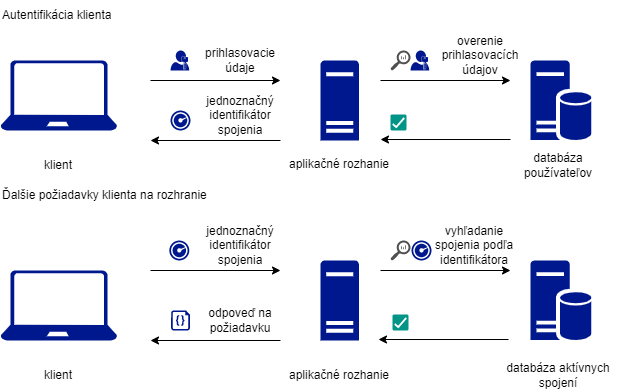
\includegraphics[width=0.8\textwidth]{images/session_schema}}
    %popis obrazku
    \caption[Schéma s použitím identifikátora spojenia]{Autentifikačná schéma s použitím identifikátora spojenia.}
    %id obrazku, pomocou ktoreho sa budeme na obrazok odvolavat
    \label{obr:session}
\end{figure}

\section{Schéma zabezpečenia využívajúca API kľuče}

API kľúč je identifikátor používaný na pripojenie k rozhraniu. Identifikuje však aplikáciu alebo službu, nie konkrétneho používateľa. Ak potrebuje aplikácia používať rozhranie, ktoré nie je verejné a na autentifikáciu používa API kľúče, musí si najprv vyžiadať API kľuč a následne ho posielať s každou požiadavkou.

Tento kľúč môže byť zároveň spojený s právami umožňujúcimi vykonávať určité volania, ak dané rozhranie poskytuje rôzne úrovne prístupu.

Použitie API kľúčov nie je veľmi bezpečné, lebo kľúče majú neobmedzenú platnosť a ak príde k ich odchyteniu, jediný spôsob ako zvrátiť ich zneužitie je ich zneplatniť a vygenerovať nové. Ďalšia zraniteľnosť API kľúčov často nastáva pri ich uložení na nesprávne miesto.

Napríklad pri webovej aplikácii nie je bezpečné ukladať kľúč na klientskej strane, ale na serveri a odtiaľ vykonávať API volania. Rovnako pri mobilnej aplikácii nie je bezpečné ukladať kľúč priamo v aplikácii, lebo sa dá získať reverzným inžinierstvom. \cite{api_key_vulnerabilities}

Preto sa vo všeobecnosti API kľúče nepoužívajú na ochranu kritických alebo citlivých volaní a zdrojov rozhrania. Naopak vhodné sú na zvýšenie kontroly nad požiadavkami na rozhranie. Je ľahké pomocou nich kontrolovať frekvenciu, či absolútny počet volaní a prípadne monetizovať ich používanie.


\section{Schéma zabezpečenia využívajúca API tokeny}

API token (ďalej token) je identifikátor, ktorý slúži na autorizáciu prípadne aj identifikáciu používateľa pri prístupe k rozhraniu. Token môže mať viaceré podoby, jednotlivým typom a formátom sa venujú podkapitoly \ref{sec:types} a \ref{sec:formats}.

Tok v rámci schémy zabezpečenia rozhrania funguje podobne ako pri využití identifikátora spojenia, ktorý sme popísali v podkapitole \ref{sec:session}. Líši sa najmä v tom, že token môže niesť pridanú informáciu a rozhranie vie jeho platnosť overiť bezstavovo. Na dosiahnutie tejto výhody je nutné použiť štruktúrovaný formát tokenu. Možné formáty tokenov detailnejšie popíšeme v podkapitole \ref{sec:formats}.


\begin{figure}
    %vlozenie samotneho obrazku vycentrovaneho a vhodnej velkosti
    %obrazok je v subore images/session.png
    \centerline{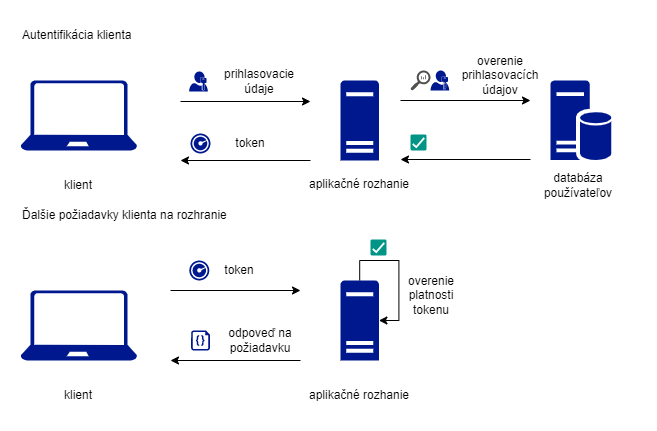
\includegraphics[width=0.8\textwidth]{images/token_schema}}
    %popis obrazku
    \caption[Schéma s použitím tokenu]{Autentifikačná schéma s použitím tokenu.}
    %id obrazku, pomocou ktoreho sa budeme na obrazok odvolavat
    \label{obr:session}
\end{figure}

\section{Typy tokenov}
\label{sec:types}

Tokeny využívané v schéme zabezpečenia rozhrania sa dajú rozdeliť podľa ich generického využitia na niekoľko typov. Nie v každom scenári máme explicitne dané aký token využiť, no niektoré sú často vhodnejšie ako iné. V tejto kapitole predstavíme viaceré typy tokenov a to prístupový (angl. access), nositeľský (angl. bearer), obnovovací (angl. refresh) a identifikačný token.

\subsection{Prístupový token}

Prístupový token \cite{access_token} je najzákladnejší a najčastejšie používaný typ tokenu. Tento token vygeneruje autentifikačný server po autentifikácii používateľa a ďalej slúži na autorizáciu v rozsahu ako sa určil v rámci autentifikácie konkrétneho používateľa. Prístupový token môže mať rôzne formáty podľa toho ako funguje schéma zabezpečenia rozhrania.

Token je spojený s istými údajmi o používateľovi ako napríklad identifikátor a prístupové práva. Tieto údaje môžu byť uložené priamo v tokene alebo na serveri, v závislosti od toho aký formát tokenu je použitý. Zároveň je s tokenom spojený aj časový limit platnosti tokenu, ktorý býva kvôli bezpečnosti krátky. Po odchytení tokenu totiž môže útočník vystupovať v mene používateľa, ktorého údaje sú uložené v tokene.


\subsection{Nositeľský token}

Nositeľský token reprezentuje najčastejší spôsob použitia prístupového tokenu. Pri jeho použití má nositeľ tokenu prístup k rozhraniu bez ohľadu nato, kto je. Stačí aby v požiadavke poslal platný nositeľský token.

Následne rozhranie nekontroluje identitu používateľa, ale iba platnosť tokenu. Preto pri jeho využití treba prikladať väčší dôraz na bezpečnosť tokenu napríklad tak, že jeho platnosť bude veľmi krátka, napríklad 5 minút.


\subsection{Obnovovací token}

Ako sme už spomínali vyššie má prístupový token často relatívne krátky časový limit platnosti. Ak chce používateľ využívať rozhranie aj po jeho uplynutí, je potrebné aby získal nový prístupový token.

Na riešenie tohto problému existujú dva jednoduché spôsoby. Buď sa používateľ znova autentifikuje a server mu vygeneruje nový prístupový token alebo si klient, cez ktorého používateľ komunikuje s rozhraním bude pamätať prihlasovacie údaje používateľa a využije ich na znovuautentifikáciu používateľa. Oba prístupy nie sú ideálne, prvá možnosť je nekomfortná pre používateľa a nie je možná ak je klientom nejaký servis alebo iná aplikácia. Druhá možnosť je nebezpečná, lebo klient musí mať niekde uložené prihlasovacie údaje používateľa a tým sa zvyšuje riziko ich získania útočníkom.

Obnovovací token adresuje problém s krátkou platnosťou prístupových tokenov. Pri prvotnej autentifikácii používateľa server okrem prístupového tokenu vygeneruje aj obnovovací token. Oba tokeny vráti klientovi. Následne keď uplynie platnosť prístupového tokenu, klient pošle požiadavku o nový prístupový token pomocou obnovovacieho tokenu. 

Schému s obnovovacími tokenmi využíva napríklad populárny autentifikačný protokol OAuth 2.0 \cite{oauth2}.


\subsection{Identifikačný token}

Identifikačný token je špeciálny typ prístupového tokenu. V tomto prípade musí ísť o štruktúrovaný formát tokenu. Token obsahuje identifikátor používateľa a autorizačné údaje. Navyše môže token obsahovať doplnkové údaje ako vydavateľa tokenu, čas platnosti tokenu, čas vydania tokenu a podobne.

Identifikačný token využíva napríklad protokol OpenID Connect (OIDC), čo je nadstavba protokolu OAuth 2.0 o identitu používateľa \cite{oidc}. OIDC dokonca presne špecifikuje použitie JWT (JSON Web Token), ktorý viac predstavíme v kapitole \ref{kap:typy}.


\section{Formáty tokenov}
\label{sec:formats}

Už sme spomenuli, že existujú rôzne typy tokenov, no iba pri identifikačnom tokene je striktne daný formát tokenu. Pri ostatných typoch sa stretávame s rôznymi formátmi tokenu. Vo všeobecnosti rozoznávame dva formáty tokenov a to nepriehľadné (angl. opaque) a štruktúrované. Existujú aj hybridné formáty, ktoré kombinujú výhody obidvoch spomínaných typov, no pri nich sa dá hovoriť skôr o istých vzoroch ako o formátoch. Najpoužívanejšie sú fantómové a rozdelené (angl. split) tokeny. 

\subsection{Nepriehľadný token}

Ide o najjednoduchší formát tokenu. Nepriehľadný token je náhodný reťazec znakov. Jednoduchý je v tom, že nenesie žiadnu pridanú informáciu pre rozhranie. Všetky metadáta o tokene si musí pamätať rozhranie.

Takýto prístup so sebou nesie významné výhody aj nevýhody. Výhodou je, že samotné vytvorenie tokenu je veľmi rýchle, rozhranie jednoducho vygeneruje náhodný reťazec. Navyše vďaka tomu, že nenesie žiadne pridané informácie, nenesie ani citlivé informácie o používateľovi, teda jeho zachytenie útočníkom nie je také nebezpečné. Nevýhodou však je, že rozhranie ho nevie bezstavovo overiť, teda ho musí napríklad vyhľadať v databáze platných tokenov a to je časovo náročné.


\subsection{Štruktúrovaný token}


Na rozdiel od nepriehľadného tokenu štruktúrovaný token obsahuje pridanú informáciu napríklad identifikáciu používateľa, jeho prístupové práva, čas platnosti tokenu, čas vydania tokenu a podobne.

Aby sa predišlo úniku citlivých informácií z tokenu, je token šifrovaný alebo zahešovaný. Využívajú sa rôzne symetrické aj asymetrické algoritmy. Všetky konkrétne protokoly, ktoré rozoberáme v tejto práci, používajú štruktúrované tokeny a v kapitole \ref{kap:typy} sa venujeme ich vytváraniu a s ním spojenému šifrovaniu alebo hešovaniu tokenov.

Najväčšou výhodou štruktúrovaného tokenu je, že rozhranie ho môže bezstavovo overiť, lebo pozná kľúč, ktorým bol token zašifrovaný alebo zahešovaný, teda ho vie dešifrovať a prečítať informácie, ktoré nesie. Zo získaných informácií vie rozhranie overiť platnosť tokenu a autorizovať používateľa.


\subsection{Fantómový token}

Ako sme naznačili v úvode podkapitoly, fantómový token \cite{phantom_token} je hybridný formát tokenu. Podľa tohto vzoru autentifikačný server vygeneruje dva tokeny, nepriehľadný token pre klienta a štruktúrovaný token pre rozhranie. Ďalej sa využíva API brána alebo reverzný proxy server (RPS), v ktorom sa uloží dvojica tokenov ako kľúč a hodnota. Kľúčom je nepriehľadný token, hodnotou je štruktúrovaný token.

Následne, keď klient pošle požiadavku na rozhranie, tak pridá nepriehľadný token. API brána alebo RPS ho preloží na štruktúrovaný token a tento štruktúrovaný token poskytne rozhraniu. Rozhranie ho môže bezstavovo overiť a využiť pridané informácie, ktoré nesie.

Brána alebo RPS síce musí vyhľadať záznam s dvojicou tokenov, kde je kľúčom poslaný nepriehľadný token, ale môže si výsledok uložiť do vyrovnávacej pamäte pre ďalšie požiadavky. Tým sa zvýši priepustnosť brány alebo RPS a zároveň ubudnú nároky na výkonnosť rozhrania.

Výhodou oproti obyčajnému štruktúrovanému tokenu je, že klient, teda prehliadač alebo iná aplikácia nedržia v pamäti štruktúrovaný token obsahujúci, aj keď zašifrované, citlivé informácie.


\subsection{Rozdelený token}

Rozdelený token \cite{split_token} má podobnú schému a výhodu ako fantómový token, no navyše ombedzuje štruktúrovaný token vydaný autentifikačným serverom tým, že musí obsahovať podpis chrániaci jeho autenticitu.

V schéme rozdeleného tokenu vydá autentifikačný server len jeden štruktúrovaný token. Podpis z tohto tokenu pošle klientovi a do vyrovnávacej pamäte brány alebo RPS zapíše celý token so zahešovaným podpisom ako kľúčom.

Požiadavky od klienta budú obsahovať ako nepriehľadný token získaný podpis a brána alebo RPS ho zahešuje a preloží na štruktúrovaný token pomocou vyrovnávacej pamäte. Token následne spolu s požiadavkou pošle rozhraniu.